\documentclass[11pt]{article}
\usepackage[margin=1in]{geometry}
\usepackage{amsmath,amssymb,amsthm,booktabs,graphicx}
\usepackage[hidelinks]{hyperref}
\makeatletter
\let\inputrows\@@input
\makeatother
\newtheorem{theorem}{Theorem}
\newtheorem{proposition}[theorem]{Proposition}
\newtheorem{corollary}[theorem]{Corollary}
\newcommand{\R}{\mathbb R}
\newcommand{\E}{\mathbb E}
\newcommand{\Prob}{\mathbb P}
\newcommand{\norm}[1]{\lVert #1\rVert}
\newcommand{\tr}{\operatorname{tr}}
\newcommand{\diag}{\operatorname{diag}}
\newcommand{\Var}{\operatorname{Var}}
\title{How many paired measurements does conditional prediction require?}
\author{Yunjie Guo \and Hanqing Yang\thanks{Corresponding author: \texttt{hanqing.yang189@gmail.com}. Affiliation of both authors: Independent Researcher, Suzhou, China.}}
\date{}
\begin{document}
\maketitle
\begin{abstract}
A sensor archive and a separate archive of scalar targets identify two Gaussian marginals while leaving their dependence undetermined. Suppose each new calibration object supplies the target and one linear instrument reading. How many such objects suffice for conditional prediction? We characterize minimax interval length up to constants for every realized archive of scores and every deployment query. For a reusable design this yields a spectral allocation problem. An integer allocation attains the optimal order against arbitrary preassigned linear directions. With unit sensor gain in $p$ dimensions, keeping the average pointwise minimax length bounded requires order $p^2$ calibration objects for a reusable archive and order $p$ for an archive acquired for one known query. We also give the exact shortest interval without pairs and a one-tail approximation with a computable error bound. For 16 Gaussian queries in 64 dimensions sharing 256 pairs, tailoring the directions to the batch reduces the mean root mean squared half-width from 8.25 to 4.39 target standard deviations. Beyond simulations with eight measured blur operators, 95\% intervals trained on spatially separate strips achieve 97.0\% and 56.8\% empirical coverage on two airborne spectral images at 256 pairs. This variation limits transfer of the model-based coverage guarantee.
\end{abstract}

\section{A missing channel}
Consider two archives of the same population of objects. A visible field was acquired in the first archive. A scalar feature of another channel, such as a coefficient in an unobserved band, was acquired in the second. At deployment a sensor returns a noisy linear measurement of the visible field. The question is how precisely one can predict the feature for this particular object. Even perfect knowledge of each archive's distribution leaves the dependence between the two fields open. A joint prior chosen by a learning procedure makes one such dependence assumption. Its posterior may be much narrower than the range supported by the archives.

A laboratory might take one extra scalar reading on each object sent for a target assay. It can decide in advance which direction each instrument should record, or it can choose a direction for an object of immediate interest and then collect calibration pairs. For a Gaussian field with $p$ unit-gain coordinates, the first option must spend order $p^2$ pairs to keep its average pointwise minimax width bounded. The second spends order $p$ per query. Section~\ref{sec:finite} derives the general spectral law and gives a discrete allocation with a finite-budget guarantee. The proof compares all preassigned unit linear directions, including oblique ones. For weakly visible fields it is the spectrum of the sensor that determines the cost.

Azizyan, Krishnamurthy and Singh establish minimax bounds for estimating a full covariance matrix from random projections of each object \cite{compressive}. Our calibration object supplies a projected field and a separate target, and the loss is conditional prediction length for that target. Incomplete-measurement learning has been studied through identifiability of signal models under multiple sensing operators \cite{tachella}. Statistical matching describes the feasible Gaussian completions of unpaired data and draws inferences about their parameters \cite{ahfock}. Chernozhukov, W\"uthrich and Zhu \cite{cwz} take the union of conditional prediction intervals over a plausible set of Gaussian copulas. Their scalar example supplies a direct benchmark for this paper. Folded-normal critical values also occur in inference with bounded bias \cite{ak}. Gaussian two-sided chance constraints have a convex representation. The robust formulation of Lubin et al.\ \cite{lubin} treats separable mean and covariance uncertainty in their tractability lemma. Our problem couples the feasible bias and conditional variance through the same latent correlation vector. Optimizing the two tails jointly gives a shorter interval than the equal-tail union can generally provide. We quantify that difference as well as the usually larger effect of acquiring paired information.

We study deterministic intervals, a scalar target and pointwise coverage over a specified class of jointly Gaussian populations. Population marginals and noise parameters are given. This isolates ambiguity that would persist with arbitrarily large unpaired archives. The prediction target can also be the residual of a missing linear functional after subtracting an identified contribution. When the target is a known functional of the visible field, its coupling is already specified. The usual Gaussian inverse problem then gives the conditional law directly.

\section{Measurement model and coverage}
Let the whitened latent field $X\sim N(0,I_p)$ and target $T\sim N(0,1)$ have unknown joint Gaussian law. Write
\begin{equation}
 T=u^\top X+\sqrt{1-\norm{u}^2}\,Z,\qquad \norm{u}\le1,\quad Z\sim N(0,1)
 \label{eq:model}
\end{equation}
with independent $Z$. Positive semidefiniteness of the joint covariance is equivalent to this unit-ball constraint, and every vector in the ball induces the same two marginal laws. Singular completions are included by continuity. For a visible signal with known covariance and colored noise, first multiply the forward operator by the signal covariance square root on the right and whiten the noise on the left. In its right singular basis, let $s_i$ be the singular values. Standardizing each left singular coordinate of the observation gives $W\sim N(0,I)$ with $\operatorname{Cov}(X,W)=D=\diag(d_i)$ and $d_i=s_i/\sqrt{1+s_i^2}$. We pad null directions with independent noise coordinates if necessary. Explicitly $W=DX+(I-D^2)^{1/2}\epsilon$ with standard Gaussian $\epsilon$ independent of $(X,T)$. Unit gains allow noiseless observations. For $W=w$ define $g=Dw$ and $M=\norm{g}$. In particular $g=\E[X\mid W=w]$. Gaussian conditioning gives
\begin{equation}
 T\mid W=w,u\ \sim\ N(u^\top g,\,1-\norm{Du}^2).
 \label{eq:conditional}
\end{equation}
Regression on any common, fully observed Gaussian covariates reduces to this model after centering and whitening the two residuals. Target units are restored by multiplying by its residual standard deviation and adding its residualization offset.

Fix $0<\alpha<1/2$, $z=\Phi^{-1}(1-\alpha/2)$ and $z_1=\Phi^{-1}(1-\alpha)$. Let $F(m,s)$ be the $(1-\alpha)$ quantile of $|m+sZ|$ for $m,s\ge0$. At $s=0$, $F(m,0)=m$. We require $\Prob_u(T\in I(w)\mid W=w)\ge1-\alpha$ for every $u$ at each $w$, using the Gaussian conditional kernel in \eqref{eq:conditional}.

We first ask how much new information can be acquired at a given budget. We then return to the exact interval available when no paired archive exists. The folded quantile $F$ is nondecreasing in its two nonnegative arguments at the levels considered here, as shown in the proof of Theorem~\ref{thm:sharp}.

\section{What can a finite reusable archive buy?}\label{sec:finite}
Suppose a calibration object supplies its target and one scalar instrument reading. Different objects can be measured in different directions. This section counts objects and scores together: an archive of size $N$ always contains $N$ targets and $N$ scalar readings. In particular an archive containing full vector observations at that price would describe a different experiment.

Object $j$ has an independent copy $(X_j,T_j)$ of \eqref{eq:model}. Its standardized reading is
\[
 S_j=c_j q_j^\top X_j+\sqrt{1-c_j^2}\,\xi_j,\qquad
 \norm{q_j}=1,\quad 0\le c_j\le1 ,
\]
with independent standard normal instrument errors. The known reliability $c_j$ may differ across instruments. A reusable design selects all directions before the deployment observation. A query-specific design can select them using $w$. Both select them before observing calibration data; independent randomization is allowed. Conditional on the scores and $w$, the calibration responses are independent with means $(Au)_j$ and variances $1-c_j^2(q_j^\top u)^2$, where row $j$ of $A$ is $c_j S_j q_j^\top$. Thus even the conditional calibration variances depend on the unidentified coupling.

Let $\ell(A,g)$ denote the infimum, over prediction intervals honest for every $\norm u\le1$, of their worst conditional expected length, with the score design understood. The expectation includes calibration responses and the new target; $(S,w)$ and the selected instruments are held fixed. Our design risk averages this \emph{pointwise minimax length} over scores, queries and any design randomization. This order of quantifiers protects each realized query and archive of scores. Marginal coverage alone would permit the constant half-width $z$ with no paired data.

\begin{theorem}[Finite-archive information]\label{thm:archive}
Set $K=I+A^\top A$ and $R^2=g^\top K^{-1}g$. Uniformly in dimension, score values, query and design,
\[
 \ell(A,g)\asymp_\alpha 1+R.
\]
An honest interval has center $t^\top T_{\rm cal}$ and half-width
\begin{equation}
 F\!\left(\norm{r},\sqrt{1+\norm t^2}\right),\qquad r=K^{-1}g,\quad t=Ar.
 \label{eq:ridge}
\end{equation}
\end{theorem}
\begin{proof}
The prediction error at that center has mean $r^\top u$ since $g-A^\top t=r$. Its variance is
\[
 1-\norm{Du}^2+\sum_j t_j^2\{1-c_j^2(q_j^\top u)^2\}\le 1+\norm t^2 .
\]
Monotonicity of $F$ proves coverage. The identity $\norm r^2+\norm t^2=R^2$ gives the upper order using $F(m,s)\le m+zs$. This ridge choice also minimizes $\norm{g-A^\top t}^2+\norm t^2$.

For the lower bound let $R>0$ and choose $v=\kappa K^{-1}g/R$. Then $\norm v^2+\norm{Av}^2=\kappa^2$ and $v^\top g=\kappa R$. At $u=\pm v$ the calibration covariance is the same diagonal matrix $\Sigma$ with entries at least $1-\kappa^2$. The total variation distance between the two calibration experiments is $2\Phi(\norm{\Sigma^{-1/2}Av})-1$, at most $2\Phi(\kappa/\sqrt{1-\kappa^2})-1$. Couple the two archives to coincide on their common mass and use identical centered prediction errors for the two targets. As in Theorem~\ref{thm:query}, the same interval must span $2\kappa R$ with probability at least $1-2\alpha$ minus that distance. A sufficiently small fixed $\kappa>0$ makes this probability positive. At $u=0$ Jensen's bound from Theorem~\ref{thm:query} gives expected length at least $2z$, including when $R=0$.
\end{proof}
The proof uses the optimal-recovery modulus and two-point reasoning familiar from inference for linear functionals \cite{donoho}. The experiment here has parameter-dependent calibration variances, an additional target draw and a random deployment functional $g$. Its information matrix is observable before opening any calibration labels. This permits a design comparison with the same budget on both sides.

\begin{theorem}[Reusable versus query-specific scalar acquisition]\label{thm:budget}
Allow all unit directions with exact calibration readings ($c_j=1$). For a reusable design with $N$ objects define
\begin{equation}
 V_D(N)=\min_{x_i\ge0,\ \sum_i x_i\le N}\sum_i\frac{d_i^2}{1+x_i}.
 \label{eq:water}
\end{equation}
The infimum of the design risk $\mathbb E\,\ell(A,DW)$ over all reusable designs is of order $1+\sqrt{V_D(N)}$. In contrast, for a query-specific design the optimal risk is of order $1+\mathbb E\norm{DW}/\sqrt{1+N}$. Constants depend only on $\alpha$. If $D=I_p$, the corresponding rates are
\[
 1+\frac{p}{\sqrt{p+N}}\quad\hbox{and}\quad 1+\sqrt{\frac{p}{1+N}}.
\]
A bounded risk as $p$ grows requires and suffices to have $N=\Omega(p^2)$ and $N=\Omega(p)$, respectively.
\end{theorem}
\begin{proof}
First fix $g$. The map $K\mapsto\sqrt{g^\top K^{-1}g}$ is convex on positive definite matrices. It is the supremum over $g^\top h\ge0$, $h\ne0$, of $(g^\top h)/\sqrt{h^\top Kh}$. For a reusable design Jensen's inequality over the independent calibration scores and instruments gives $\mathbb E[R\mid g]\ge\sqrt{g^\top(I+J)^{-1}g}$, $J=\mathbb E[A^\top A]$, with $\tr J\le N$. For a standard normal $W$ and positive semidefinite $C$, $\mathbb E\sqrt{W^\top C W}\ge\sqrt{2/\pi}\sqrt{\tr C}$. Diagonalize $C$ and apply concavity of the square root with weights equal to the normalized eigenvalues. Hence the mean radius is at least a constant times $\sqrt{\tr[D^2(I+J)^{-1}]}$. By Cauchy--Schwarz, diagonal element $i$ of $(I+J)^{-1}$ is at least $1/(1+J_{ii})$. This proves the lower bound over arbitrary oblique designs, including less reliable unit instruments.

For achievability take a minimizer $x$ of \eqref{eq:water}, assign $\lfloor x_i\rfloor$ objects to eigenaxis $i$ and distribute any remaining observations. With $n_i$ independent objects along that axis its information is $\chi^2_{n_i}$ (zero if $n_i=0$). Write $v(n)=\mathbb E(1+\chi^2_n)^{-1}$. For $n=\lfloor x\rfloor\le3$, $v(n)\le1\le5/(1+x)$. For $n\ge4$, $v(n)\le\mathbb E[(\chi^2_n)^{-1}]=1/(n-2)\le5/(1+x)$. Consequently $\mathbb E R^2\le5 V_D(N)$; apply Jensen's upper bound and Theorem~\ref{thm:archive}.

For any query-specific design $R\ge\norm g/\sqrt{1+\tr(A^\top A)}$. Conditional on $g$, Jensen's inequality and the budget bound the mean below by $\norm g/\sqrt{1+N}$. Repeating $q=g/\norm g$ gives $R^2=\norm g^2/(1+\chi^2_N)$ and the inverse-moment bound gives the matching order. Take any direction if $g=0$. For $D=I_p$, \eqref{eq:water} has $x_i=N/p$ and $\mathbb E\norm W\asymp\sqrt p$.
\end{proof}
The two rates refer to one new query evaluated under the two acquisition rules. A reusable archive serves future queries without further pairs. Applying the query-specific guarantee to many independent queries can require a new archive for each one. Neither statement permits a repeated calibration target to count as several independent objects.

\paragraph{How attenuation changes the budget.}
For gains $d_i=i^{-\beta}$, $0\le\beta<1/2$, the reusable budget needed for bounded risk is of order $p^{2-2\beta}$, and the single-query budget is of order $p^{1-2\beta}$. At $\beta=1/2$ these thresholds become $p$ and $\log p$ respectively. For $\beta>1/2$, bounded risk is already possible at zero budget. To verify the thresholds, let $s=\sum_i d_i$. Cauchy--Schwarz gives $V_D(N)\ge s^2/(p+N)$; taking $x_i=Nd_i/s$ gives $V_D(N)\le s^2/N$ for $N>0$. These bounds suffice below $\beta=1/2$, where $s^2/p$ diverges. At the boundary, for $1\le N<p$ use $(1+x_i)^{-1}\ge1-x_i$ on $i>N$ to obtain
\[
 V_D(N)\ge\sum_{i=N+1}^p i^{-1}-N/(N+1).
\]
This quantity diverges if $N=o(p)$. The single-query assertions follow from $\mathbb E\norm{DW}\asymp(\sum_i d_i^2)^{1/2}$, and $V_D(0)=\sum_i d_i^2$ gives the last case.

\paragraph{An implementable allocation.}
For positive $N$ and some nonzero gain, the solution of \eqref{eq:water} is $x_i=(d_i/\tau-1)_+$ with $\tau$ chosen to exhaust the budget, by the first-order conditions. Proportional allocation to all gains omits the threshold for weak directions. One can also minimize $\mathbb E R^2$ \emph{exactly within the eigenaxis catalogue} even with known mode-specific reliabilities. For $n$ past observations of axis $i$, put
\[
 v_i(n)=\mathbb E[(1+c_i^2\chi^2_n)^{-1}]
       =\int_0^\infty e^{-t}(1+2c_i^2 t)^{-n/2}\,dt .
\]
Tonelli's theorem and the Laplace transform of a chi-square give the equality. The expected squared modulus is $\sum_i d_i^2 v_i(n_i)$. Each extra object's benefit $d_i^2[v_i(n_i)-v_i(n_i+1)]$ is nonnegative and decreases in $n_i$, directly under the integral. The separable resource allocation principle \cite{greedy} applies to these particular chi-square returns. Choosing the largest available benefit at each step takes the largest $N$ benefits subject to their prefix order, and hence gives an optimal integer allocation. With unit reliabilities it inherits the constant-factor length guarantee against every reusable oblique design from Theorem~\ref{thm:budget}. Exact optimality here applies to the squared modulus in the catalogue; the length guarantee against unrestricted designs is up to constants. This distinguishes the criterion from linear-regression excess prediction loss under limited attribute observation \cite{budgetlearn} and relates \eqref{eq:water} to trace criteria in Bayesian design \cite{aoptimal}.

\begin{corollary}[One archive for a known batch]\label{cor:batch}
Suppose the visible measurements for $m$ queries arrive together, before a single archive of $N$ pairs is acquired. Let $G$ have rows $g_h^\top$ and let $\sigma_i$ be the singular values of $G/\sqrt m$, padded with zeros. The best root mean square of conditional minimax lengths over the batch and calibration scores satisfies
\[
 \inf_{\rm design}\left\{\frac1m\sum_{h=1}^m
 \mathbb E_S\,\ell(A,g_h)^2\right\}^{1/2}
 \asymp_\alpha 1+\sqrt{V_{\diag(\sigma)}(N)} .
\]
The design may use all the visible queries and has no access to their targets. The discrete allocation above, in the right singular basis of the batch with weights $\sigma_i^2$, attains this order. For $m\le p$ orthogonal query vectors of norm $\sqrt p$, the squared-modulus criterion in the relaxation equals $p/(1+N/m)$. Thus the budget needed for bounded RMS length grows as $mp$ in this example.
\end{corollary}
\begin{proof}
The sum of squared moduli divided by $m$ is $\tr(C K^{-1})$ with $C=G^\top G/m$. For each row Jensen's inequality as in Theorem~\ref{thm:budget}, followed by squaring, gives $\mathbb E_S R_h^2\ge g_h^\top(I+J)^{-1}g_h$. Diagonalize $C$, use the diagonal inverse bound in that basis, and apply $\tr J\le N$. Rounding the relaxed allocation and applying the chi-square bound in the same basis achieves the matching upper order. The orthogonal example has $m$ equal nonzero eigenvalues $p/m$. The criteria average individually honest lengths; they specify no joint event of simultaneous coverage.
\end{proof}
The trace criterion for a known batch also occurs in transductive experimental design. Yu, Bi and Tresp minimize predictive variance on specified test inputs in regularized regression \cite{transductive}. Here its connection to honest interval length follows from the lower and upper bounds in Theorem~\ref{thm:archive}; the chosen instrument fixes a direction, while the scalar score realized on each new object supplies random information along it. Repeated or nearly collinear queries can share calibration, even when their number is large. Classical design for a specified linear functional also orients measurements toward the target \cite{elfving}; here the spectrum of the observed batch determines the robust prediction cost while calibration variances remain unidentified.


\section{Exact interval with unpaired archives}
\begin{theorem}[Sharp radius and scalar dual]\label{thm:sharp}
A shortest interval is $[-H,H]$, where
\begin{equation}
 H=\max_{\norm{u}\le1} F\bigl(|u^\top g|,\sqrt{1-\norm{Du}^2}\bigr).
 \label{eq:radius}
\end{equation}
Write $f(t)=F(t,1)$ for $t\ge0$. Define $k(a)=f(t)-at$ at $a=f'(t)$ and extend by $k(0)=z$, $k(1)=z_1$. For $0\le a\le1$, $k>0$, set
\begin{equation}
 L(a,k)^2=\min_{0\le\lambda<1}
 \left\{\sum_{i:d_i>0}\frac{a^2g_i^2}{\lambda+(1-\lambda)d_i^2}
              +\frac{k^2}{1-\lambda}\right\}.
 \label{eq:dual}
\end{equation}
Then $H=\max_{a\in[0,1]} L(a,k(a))$. The half-length of the union of central equal-tail intervals is $L(1,z)$.
\end{theorem}
\begin{proof}
For fixed half-length, Gaussian interval mass decreases with the distance between its center and the mean. The two completions $u$ and $-u$ have equal variance and opposite means. For any center $c$, at least one distance is at least $|u^\top g|$. Recentring at zero therefore weakly improves the minimum coverage for each pair. This argument also applies to point masses. Compactness and continuity give attainment in \eqref{eq:radius}.

The quantile equation is $\Phi(f-t)+\Phi(f+t)=2-\alpha$. Implicit differentiation gives $f'(t)=\tanh(tf(t))$ and $f''(t)=(1-f'(t)^2)(f(t)+tf'(t))>0$. Also $f(t)-t\to z_1$, by the quantile equation, and $t(1-f'(t))\to0$. Thus $k(a)$ decreases continuously from $z$ to $z_1$, with derivative $-t$ in the interior. Supporting tangents and homogeneity imply
\[
 F(m,s)=\max_{0\le a\le1}\{am+k(a)s\}.
\]
In particular $F$ increases weakly in both arguments. The two maxima in \eqref{eq:radius} commute. At a fixed tangent, use the sign symmetry and introduce $v\ge0$. Maximize $a g^\top u + kv$ subject to $\norm{u}^2\le1$ and $\norm{Du}^2+v^2\le1$. A convex combination of the constraints with weights $\lambda,1-\lambda$ and Cauchy--Schwarz gives \eqref{eq:dual} as an upper bound. Null coordinates can be set to zero.

For equality put $B_i=\lambda+(1-\lambda)d_i^2$ and let $L$ be the square root of the minimized expression. Take $u_i=ag_i/(LB_i)$, $v=k/[L(1-\lambda)]$. This attains equality on the combined ellipsoid. The derivative of the expression under the minimum is $L^2(\norm{Du}^2+v^2-\norm{u}^2)$ evaluated at the minimizing $\lambda$. An interior minimum makes both constraints tight. At zero the right derivative is nonnegative, so the first constraint is satisfied and the second is tight. The objective diverges as $\lambda\uparrow1$. This proves equality. Finally the largest equal-tail endpoint is the support with coefficients $(1,z)$. The union is an interval since the family of central intervals varies continuously over a connected ball.
\end{proof}

\paragraph{Computing an interval and its witness.}
The dual objective is convex in $\lambda$. Its derivative gives either the left endpoint or a scalar root. An outer subinterval $[a_0,a_1]$ has upper bound $L(a_1,k(a_0))$ since $L$ is increasing in each coefficient. Evaluating feasible $u$ at a tangent gives a lower bound directly from \eqref{eq:radius}. Bisect the subinterval with the largest upper bound until the gap is within tolerance. Continuity on the compact slope interval implies termination at any positive tolerance in exact arithmetic. This construction requires sums in singular coordinates and scalar root searches. The implementation uses double precision and returns both endpoints and the witness. For a single noiseless coordinate the equal-tail union is $\sqrt{w^2+z^2}$. At $w=0$ the sharp answer is $z$. For $g\ne0$ and $d_i<1$ for all $i$, the union is strictly wider. Indeed its radius exceeds $z$ by taking a small step from zero along $g$. At a maximizer of the sharp radius, either the mean is zero and the radius is at most $z$, or the mean is positive and its folded quantile is strictly below the equal-tail endpoint $m+zs$.

\paragraph{A single-support comparison.}
Let $B_0=\max\{z,L(1,z_1)\}$ and let $\phi$ be the standard normal density. A simpler bracket, using one support evaluation, is
\begin{equation}
 B_0\le H\le B_0+\Phi(-B_0)/\phi(z).
 \label{eq:tail}
\end{equation}
Indeed, requiring each tail to have probability at most $\alpha$ gives $H\ge m+z_1s$ for every feasible absolute mean $m$ and standard deviation $s$. Set $\eta=\Phi(-B_0)\le\alpha/2$. Moving the normal quantile from $1-\alpha$ to $1-\alpha+\eta$ costs at most $\eta/\phi(z)$ by the mean value theorem. Since $s\le1$, the upper endpoint in \eqref{eq:tail} spends at most $\alpha-\eta$ on the near tail and at most $\eta$ on the far tail. The minimum of this upper bound and the equal-tail union is also valid. The exact formula can improve the most when the observation leaves appreciable mass in both tails; Appendix~\ref{app:bench} checks that regime.

\begin{corollary}[Effective dimension]\label{cor:dimension}
For $m_D=\tr D^2$,
\[
 \max(z,M)\le H\le M+z,\qquad
 \E[M^2]=m_D,\quad \Var(M^2)=2\tr D^4.
\]
Along any sequence with $m_D\to\infty$, $H/\sqrt{m_D}\to1$ in probability and in mean.
\end{corollary}
\begin{proof}
Use $u=0$ and, for $M>0$, $u=g/M$ in \eqref{eq:radius}. Since $1-\alpha>1/2$, $F(m,s)\ge m$. The triangle inequality gives $F(m,s)\le m+zs$. The random sum $M^2=\sum d_i^2W_i^2$ has the stated moments, with variance at most $2m_D$. Hence $M^2/m_D\to1$ in mean square. The bounds and $|\sqrt{x}-1|\le|x-1|$ yield the claim.
\end{proof}
The constant interval $[-z,z]$ has precisely the requested coverage after averaging over $W$ for each fixed completion. The dimension cost comes from protecting each observed $w$ against every compatible direction. The witness can differ across $w$ because each candidate interval must pass all of these pointwise tests.

\section{Benchmarks with identified projections and a single query}
Suppose a calibration study can measure the target and $k$ linear scores of the whitened latent field on the same object. These scores require access to the specified projections in calibration. A noisy deployment image alone does not provide them. A fixed design collects scores for many future objects. A query-specific design chooses one score after seeing the current measurement.

\subsection{Fixed projections}
Let $P$ be a rank-$k$ orthogonal projector and $Q=I-P$. Start with a population calibration archive that identifies $b=Pu$ exactly. Possible couplings have the form $b+v$ with $v\in\operatorname{im}Q$, $\norm v\le\sqrt{1-\norm b^2}$. The possible conditional means fill the interval with midpoint $b^\top g$ and half-length $\sqrt{1-\norm b^2}\,\norm{Qg}$. Its largest expected squared half-length over $b$ is $\tr(QD^2)$. Prediction widths also depend on the residual variance.

\begin{theorem}[Optimal fixed paired subspace]\label{thm:fixed}
Order the gains $d_1\ge\cdots\ge d_p$. Let $h(P,b,w)$ be the half-length of a shortest conditionally valid interval after learning $Pu=b$. For every threshold $x$, the projector $P_*$ onto the first $k$ right singular directions minimizes
\[
 \sup_{b\in\operatorname{im}P,\,\norm b\le1}\Prob_W\{h(P,b,W)>x\}.
\]
The optimal tail probability equals that of the unpaired radius with gains $(d_{k+1},\ldots,d_p)$ and a standard normal measurement of that dimension. The optimal worst expected squared half-length of the \emph{mean range} is $\sum_{i>k}d_i^2$.
\end{theorem}
\begin{proof}
Every projector must allow $b=0$. Write $B$ for an orthonormal basis matrix of its complementary space. At $b=0$ the feasible test correlations are $DBv$ with $\norm v\le1$. Rotating the measurement and using the singular value decomposition reduces \eqref{eq:radius} in law to the spectrum of $DB$. The squared singular values are the eigenvalues of $B^\top D^2B$. By the variational characterization of eigenvalues the $j$th largest is at least $d_{k+j}^2$. In common rotated coordinates a coordinatewise larger spectrum generates a larger correlation ellipsoid $\{c=\diag(d_i)v:\norm v\le1\}$. Given $w$, the conditional mean and variance at $c$ are $c^\top w$ and $1-\norm c^2$. Nesting orders the supremum pointwise in the coupled standard normal coordinates. This proves the lower bound on every tail probability.

For $P_*$ the zero-calibration case has exactly the trailing spectrum. At any other $b$, center the interval at $b^\top g$. Relative to this center the mean is $v^\top g$, the feasible ball for $v$ shrinks and the variance is $1-\norm{Db}^2-\norm{Dv}^2$ by orthogonality in the singular basis. Monotonicity of $F$ makes the zero-calibration half-length feasible throughout. This proves attainment. Taking the trace of the compression gives the mean-range claim.
\end{proof}
Classical Gaussian optimal-information theory studies the best linear observations for average and probabilistic approximation criteria \cite{wasilkowski}. Leading singular subspaces also optimize approximations of Gaussian posteriors for a specified prior \cite{spantini}. Here the design controls all worst-case width quantiles over unknown couplings. A new paired direction contributes little if many equally informative orthogonal directions remain. In the unit-gain case $k$ fixed scores leave a typical half-length of order $\sqrt{p-k}$ whenever $p-k$ diverges.

\subsection{A projection chosen for one observation}
For $M>0$ take $q=g/M$. Learning $q^\top u$ identifies the mean in \eqref{eq:conditional}. Only $\pm q$ achieves this for all couplings using one unit direction. Any component of $g$ orthogonal to the calibration direction leaves two opposite couplings with identical calibration and different conditional means. Given $q^\top u$, a half-length of $z$ around the identified mean suffices. For $M=0$ the unpaired interval already has that width.

Choose $q$ using $w$ before drawing the calibration objects. For each of $n$ independent copies observe $S_j=q^\top X_j$ and $T_j$. Write $E=\sum_j S_j^2$, $\beta=q^\top u$, and $\widehat\beta=\sum_j S_jT_j/E$. The coverage probability below averages over the calibration responses and the new target, conditionally on $w$ and the calibration scores. Conditioning additionally on the realized calibration responses would give a different guarantee.
\begin{theorem}[Cost of query-specific pairing]\label{thm:query}
For $E>0$ a valid interval is
\begin{equation}
 M\widehat\beta\ \pm\ z\sqrt{1+M^2/E}. \label{eq:paired}
\end{equation}
At $u=0$ coverage equals $1-\alpha$. Among intervals with this center and deterministic half-length given $(w,S)$ this radius is minimal.

For any interval $I$ with the stated uniform coverage, choose $0<c<1$ such that $\eta=1-2\alpha-[2\Phi(c)-1]>0$, and set $\delta=c/\sqrt{1+E}$. At the fixed $(w,S)$ there exists a compatible coupling under which
\begin{equation}
 \Prob\{|I|\ge2\delta M\mid w,S\}\ge\eta . \label{eq:lower}
\end{equation}
The minimax conditional expected length over all valid intervals is of order $1+M/\sqrt{1+E}$, with constants depending only on $\alpha$.
\end{theorem}
\begin{proof}
Regression on the scores gives $\widehat\beta\mid S\sim N(\beta,(1-\beta^2)/E)$ independently of the new target given $w$. The prediction error has mean zero and variance
\[
 1-\norm{Du}^2 + M^2(1-\beta^2)/E.
\]
Its maximum $1+M^2/E$ is attained at $u=0$, proving the first claims.

For the lower bound use $u_+=\delta q$, $u_-=-\delta q$. The calibration response vectors have means $\pm\delta S$ and common covariance $(1-\delta^2)I$. Their total variation distance is $2\Phi(\delta\sqrt{E}/\sqrt{1-\delta^2})-1\le2\Phi(c)-1$, by integration over the half-space where one density is larger. Couple the calibration responses to be identical with probability one minus this distance, by sampling the common part of their densities first. Independently couple the two new targets with the same centered Gaussian error. They are then separated by exactly $2\delta M$. With probability at least $\eta$ the same calibration vector is seen and both targets are covered, by the union bound. On that event the interval spans their separation. This proves \eqref{eq:lower}, also for independent procedure randomization shared in the coupling.

At $u=0$ the new target is standard normal independently of calibration. A random interval of length $l$ covers with conditional probability at most $2\Phi(l/2)-1$, a concave function. Jensen's inequality gives expected length at least $2z$. For the matching upper bound use the shorter, based on $(w,S)$ alone, of the unpaired interval and \eqref{eq:paired}. For $E<1$ use $H\le M+z$, and for $E\ge1$ use \eqref{eq:paired}.
\end{proof}
Here $E\sim\chi^2_n$ and $M^2$ has mean $m_D$. As $m_D$ and $n$ diverge, both concentrate relative to their means. A bounded minimax expected length at typical scores and queries requires $n$ of order $m_D$ or larger. One \emph{type} of paired measurement resolves the mean ambiguity. Estimating its covariance can require many paired objects. This design uses fresh calibrators or existing independent paired fields from which the chosen score can be extracted. An archive of one previously chosen projection provides a different experiment.

\section{Equal-budget comparisons on simulated and measured queries}\label{sec:numerics}
We use all eight blur kernels from Levin et al.\ \cite{levin}, obtained from Bouman's laboratory materials \cite{bouman}. Each defines periodic convolution on a $32\times32$ visible field. The target is a standardized coefficient of a second, unmeasured channel. The study combines measured blur weights, specified field spectra and simulated queries. This permits a check of the radius and its coverage against a known family of compatible populations.

For Fourier indices $j,l$ put $A_{jl}=\sin^2(\pi j/32)+\sin^2(\pi l/32)$. The smooth field has spectral variance $(1+64A_{jl})^{-1}$ and the white field has variance one. Multiplying its spectral standard deviations by the modulus of the kernel transform and dividing by the noise standard deviation gives the noise-whitened singular values. A real sine--cosine basis counts each conjugate pair twice, giving 1,024 real coordinates. We use noise levels 0.05, 0.2 and 0.8. For the unpaired benchmark in Appendix~\ref{app:bench}, at the primary smooth setting with noise 0.2 we use the same 16 seeded standard normal test vectors in descending gain order for each kernel. Reuse facilitates paired comparisons and induces dependence across kernels. All intervals have nominal coverage 95\%. Half-lengths are in target standard deviations.

\subsection{Finite pairs at the same acquisition budget}
The finite experiments use \eqref{eq:ridge} with a fixed ridge parameter of one. Each archive reads one projection and one target per object. Competing policies receive the same objects and the same test queries within a replicate. The exact integer allocation chooses the largest expected decrease in squared modulus. A mean-information comparator replacing each $\chi^2_n$ by its mean $n$ would minimize $\sum_i d_i^2/(1+n_i)$; we implement its exact integer optimum by repeatedly taking the largest $d_i^2/[(1+n_i)(2+n_i)]$. We call this the mean-information allocation. Further policies round proportional shares $Nd_i/\sum d_j$, cycle through a uniformly permuted list of coordinates, or repeatedly read only the leading four. The cost model charges a single scalar projection even if its hardware requires a dense filter.

\begin{figure}[htbp]
\centering
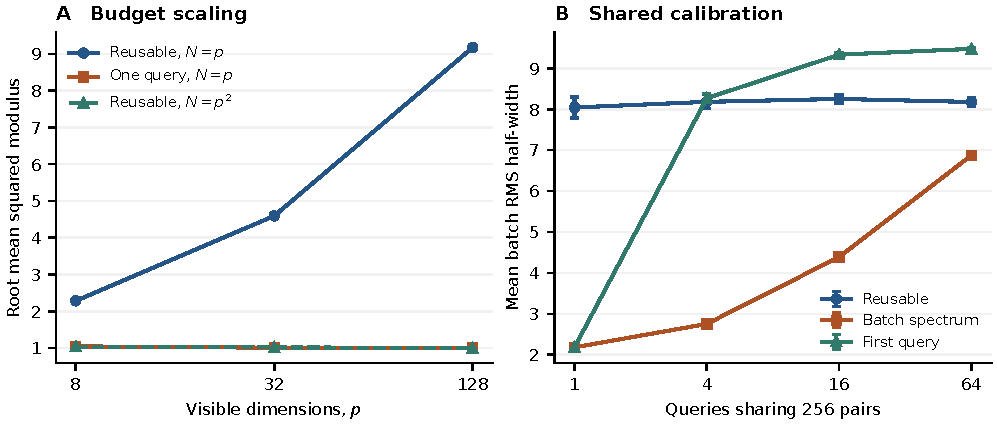
\includegraphics[width=.99\linewidth]{allocation.pdf}
\caption{Acquisition cost depends on which queries a common archive must serve. Panel A uses 512 Gaussian realizations per point. Panel B averages RMS half-width within each batch over 32 replicates at $p=64$. Bars show two Monte Carlo standard errors across independent batches. Each policy uses 256 pairs across the whole batch.}
\label{fig:allocation}
\end{figure}
At $N=p$, increasing $p$ from 8 to 128 increased the root mean squared modulus for balanced reusable acquisition from 2.28 to 9.17; the query-specific value stayed between 1.00 and 1.05. Spending $p^2$ pairs on reusable acquisition kept this modulus between 1.00 and 1.04. These values check the dimension dependence of Theorem~\ref{thm:budget}. For random batches of 16 queries in 64 dimensions with 256 shared pairs, the mean batch RMS half-width was 4.39 with the batch-spectrum design, 4.36 with mean-information allocation in that same basis, 8.25 with balanced reusable acquisition and 9.33 when all readings targeted the first query. The paired difference between reusable and batch-spectrum widths averaged 3.86 (Monte Carlo standard error 0.06). Across the 512 targets in that cell the corresponding empirical coverages were 96.5\%, 97.9\%, 98.4\% and 100\%, respectively. Learning which span must be served accounts for much of the width reduction.

We isolated the effect of allocating \emph{within} a known span in a supplemental comparison specified after the random-batch results. Each of 16 queries has norm 8 in 64 dimensions. With equal spectral energy the proposed and span-balanced schedules coincide. If one direction carries 75\% of batch energy and the other fifteen share the rest, the integer optimum assigns 76 of the 256 pairs to the leading direction. Compared with splitting the pairs equally within the same span, the integrated squared modulus falls from 4.224 to 2.067 and the RMS half-width from 4.48 to 3.44 across 256 fresh archives. The mean-information rule assigns 83 pairs to that direction, with squared modulus 2.076 and RMS half-width 3.44. The principal gain here comes from the anisotropy itself. Accounting for score-energy fluctuations makes a small difference to the allocation criterion.

\begin{table}[htbp]
\centering
\caption{Reusable archives on eight blur kernels. Columns show mean squared modulus $R^2$, mean of within-archive median half-widths $h_{50}$, and RMSE of the estimated conditional mean, averaged over archives and kernels. Each archive uses 64 held-out queries.}
\begin{tabular}{lrrrrrr}
\toprule
&\multicolumn{3}{c}{$N=32$}&\multicolumn{3}{c}{$N=256$}\\
\cmidrule(lr){2-4}\cmidrule(lr){5-7}
Allocation & $R^2$ & $h_{50}$ & RMSE & $R^2$ & $h_{50}$ & RMSE\\
\midrule
\inputrows camera_rows.tex
\bottomrule
\end{tabular}\label{tab:finitecamera}
\end{table}
The coupling in Table~\ref{tab:finitecamera} is held fixed across queries. It has norm 0.8 and equal squared loadings on the first direction and the uniform vector over the remaining coordinates. We used 16 archives per kernel and budget, and generated responses from the joint Gaussian law. At $N=256$, exact allocation reduces squared modulus from 38.00 for balanced acquisition to 20.07. Its median half-width falls from 8.59 to 7.87. At $N=32$ the ordering of actual widths reverses, despite the improvement in squared modulus. Focusing on four leading directions gives the best center RMSE for this particular coupling at both budgets. Coverage across all averaged policy-budget cells is at least 99.8\%. The table illustrates both the conservatism of the uniform half-width and the distinction between the allocation criterion and performance at one fixed population.

\subsection{Spatial holdouts with measured missing-band targets}
We used the corrected Indian Pines and Salinas AVIRIS cubes \cite{scenes}. We formed 24 visible variables by averaging successive groups of six among the first 144 retained bands. The target was the average of the last 16 retained bands at the same pixel. All pixel values and targets come from the published images. Each scene was split into four contiguous row strips. In each rotation, four disjoint strips supplied visible marginal moments, target-only moments, paired calibration objects and test targets respectively. Whitening used the visible strip alone; the target scale used the target-only strip. For deployment we added independent Gaussian noise with standard deviation 0.2 times the root mean visible-group variance. The calibration readings used the measured bands without added noise. We used every fourth test row and column, and 16 independent calibration samples at each budget. The archive for each method in a comparison contains the same pixels.

The eigenaxis designs project onto principal components of the visible-strip covariance. A band-group instrument instead reads a single one of the 24 visible groups on each paired pixel, cycling over the groups in a seeded order. In whitened coordinates its direction is the normalized loading vector of that band group. This comparator uses the same number of scalar readings and targets. Dense spectral projections and direct band readout can have different engineering costs. The study retrospectively computes both from full spectra.

\begin{table}[htbp]
\centering
\caption{Prediction of withheld measured bands. Each scene's numbers average equally over four held-out strips and 16 calibration samples per strip. Width is the mean of per-archive median half-widths. Width and RMSE use the target-only strip's standard deviation in each rotation. Coverage is empirical and reported in percent.}
\begin{tabular}{rlrrrrrr}
\toprule
& &\multicolumn{3}{c}{Indian Pines}&\multicolumn{3}{c}{Salinas}\\
\cmidrule(lr){3-5}\cmidrule(lr){6-8}
$N$&Allocation&Width&Coverage&RMSE&Width&Coverage&RMSE\\
\midrule
\inputrows scene_rows.tex
\bottomrule
\end{tabular}\label{tab:scenes}
\end{table}

For Indian Pines at 256 pairs, the exact allocation gives mean median half-width 2.34 and mean coverage 97.0\%. Its four strip coverages average 95.8--97.9\% individually over the 16 archives. Direct band groups require half-width 3.68 and cover 99.6\%. The mean-information rule gives 2.33 and 96.3\%; proportional allocation gives 2.34 and 96.5\%. Similar width for these spectral allocations limits the evidence for an advantage from the exact integer marginal returns on this scene. The marginal-only interval, centered on the separate target strip with half-width 1.96, covers 87.9\% overall, ranging from 60.1\% to 100\% across strips.

Salinas shows a substantial failure of spatial transfer. At 256 pairs the exact allocation has half-width 2.03 and empirical coverage 56.8\%. The four strip coverages are 45.8\%, 58.2\%, 97.8\% and 25.5\%. The direct band-group archive covers 70.9\% at half-width 2.59, and the target-only interval covers 45.9\%. Raising the budget from 32 to 256 narrows the exact-allocation interval from 2.50 to 2.03 while its center RMSE stays at 2.04 and coverage falls from 76.1\% to 56.8\%. More paired pixels from one strip do not ensure calibration on another. Each scene provides four spatial holdouts; the 16 archives per rotation resample calibration pixels and deployment noise around the same held-out targets. Treating them as independent scenes would understate spatial uncertainty.

We examined target marginals after seeing the coverage results. In the worst Salinas fold the held-out target mean is 2.28 target-reference standard deviations above the reference-strip mean, and its standard deviation is 1.22 times the reference value. Across the four Indian Pines folds the absolute mean shifts range from 0.41 to 1.35 standard deviations. These diagnostics document a violation of the common-marginal assumption. They do not by themselves distinguish the contributions of changing marginals, conditional structure and non-Gaussianity to the coverage errors.


\section{Scope}
The population interval quantifies uncertainty left by two unpaired marginals under joint Gaussianity. Covariances, means and sensor noise used in whitening must be known for the stated guarantees. Estimating marginal parameters adds uncertainty. Restrictions on the cross-covariance, including a known sign or locality pattern, could narrow the interval. Conversely, Gaussian marginal histograms alone give little protection. For a scalar noiseless observation, take $T=\Phi^{-1}(\pi(\Phi(W)))$ with $\pi$ a measure-preserving permutation of the unit interval. Exchanging an interior probability interval with an equal-length interval near one preserves both marginals and can move targets outside a Gaussian conditional interval on a set of positive probability. Conditional calibration under non-Gaussian dependence would need additional information.

The exact fixed-subspace result concerns known calibration covariances. The finite-archive guarantees average over calibration responses at fixed readings and test query. They permit known Gaussian measurement noise and preset instruments, including query-informed choices made before collection. Simultaneous coverage for all future objects after seeing all labels, or instrument selection driven by previous labels, would require a different analysis. The spectral allocation optimizes expected squared information radius in its eigenaxis catalogue. Matching constants for the shortest finite-archive prediction interval under general oblique designs remain open.

\paragraph{Reproducibility.}
Code, experimental protocol, input digest and numerical results accompany the article at \url{https://github.com/fightforbelief/p20-unpaired-prediction}. The implementation uses Python, NumPy and SciPy.
\paragraph{Declarations.}
The authors received no specific funding for this work and declare no competing interests.

\appendix
\section{Unpaired and single-query benchmarks}\label{app:bench}
\begin{table}[ht]
\centering
\caption{Information and uncertainty by measured kernel. The traces give the expected squared half-range of compatible means before and after learning 32 leading paired projections at zero revealed covariance. $M$, sharp and equal-tail union radii are medians across 16 observations.}
\begin{tabular}{crrrrr}
\toprule
Kernel & $m_D$ & Trailing trace & $M$ & Sharp & Union \\
\midrule
1 &41.99&20.89&6.490&7.795&8.054\\
2 &36.41&16.24&6.016&7.274&7.525\\
3 &41.31&17.34&6.273&7.451&7.686\\
4 &31.45&15.33&5.687&7.012&7.274\\
5 &54.09&30.25&7.235&8.489&8.736\\
6 &48.46&26.60&6.879&8.182&8.439\\
7 &42.53&24.12&6.438&7.770&8.030\\
8 &35.07&18.04&5.880&7.198&7.458\\
\bottomrule
\end{tabular}\label{tab:kernels}
\end{table}
Across the 128 observations the upper endpoints of the sharp numerical brackets reduce the union half-length by 2.38--4.33\%. Absolute bracket widths are below 0.0005. At the returned feasible witnesses the upper radii give conditional Gaussian coverage of 0.95004 to five decimal places. Each witness concerns its own query. The equal-tail comparison measures the cost of its tail allocation. On these same 128 queries, $B_0$ ranges from 6.279 to 9.559 and the maximum excess half-width bound in \eqref{eq:tail} is $2.92\times10^{-9}$ standard deviations. A separate implementation recomputed the inner support and checked a feasible lower witness. At this signal strength the single-support bound captures essentially the full gain. Paired data address the main source of width. For kernel 1, learning 32 leading directions cuts worst expected squared mean ambiguity from 41.99 to 20.89. Thirty-two uniformly random orthogonal scores leave 40.68 on average by rotational symmetry.

For the smooth field, reducing noise to 0.05 gives effective dimensions from 155.87 to 219.71 across kernels. Raising noise to 0.8 gives 4.30 to 9.28. For white fields the ranges at noise 0.05, 0.2 and 0.8 are 679.03--837.61, 253.18--389.72 and 38.86--63.52. Greater visibility expands the possible conditional means of the missing target when the direction linking the channels is unknown. The visible field itself is better determined by a more informative sensor.

\begin{table}[ht]
\centering
\caption{Query-specific pairing for kernel 1, first observation ($M=7.445$). Each sample size and coupling uses 50,000 independent conditional trials. Adjusted intervals use \eqref{eq:paired}. Plug-in intervals ignore calibration error and use half-length $z$. The median adjusted half-length is reported at $u=0$.}
\begin{tabular}{rrrrrr}
\toprule
& & \multicolumn{3}{c}{Adjusted coverage (\%)} & Plug-in (\%)\\
\cmidrule(lr){3-5}
$n$ & Median half-length & $u=0$ & $u=.5q$ & $u=.95q$ & $u=0$\\
\midrule
4   & 8.204 &94.95&97.75&100.00&36.51\\
16  & 4.214 &94.91&97.28&100.00&63.02\\
64  & 2.683 &95.05&96.89&99.88&84.47\\
256 & 2.162 &94.99&96.60&99.45&92.39\\
\bottomrule
\end{tabular}\label{tab:paired}
\end{table}
For this first query the unpaired radius is between 8.6840 and 8.6844. Independent calibration responses and target draws were generated using their conditional normal laws at three fixed couplings. Rounding to 100\% can hide rare misses (two in 50,000 at $n=16$, $u=.95q$). At zero coupling the Monte Carlo standard error is about 0.10 percentage points. The finite-calibration correction matters even at $n=256$. At other couplings it can be conservative because both variance terms in the proof of Theorem~\ref{thm:query} can shrink.

\subsection{When is the exact two-tail computation useful?}
To complement the high-signal blur examples, we evaluated scalar gains $d=0.5,1$ at $|w|=0,0.75,1.5,2.25,4,8$. The simple method takes the smaller of the upper bound in \eqref{eq:tail} and the union half-width. At $d=0.5$, $|w|=1.5$, the sharp, simple and equal-tail half-widths were 2.178, 2.428 and 2.447. At $d=1$, $|w|=8$, both the sharp and simple methods gave 8.167 to three decimal places, while the equal-tail union gave 8.237. All twelve cells, including the null observation where the three coincide, are archived. This comparison checks approximation error in regimes that the measured-kernel settings scarcely sample.


\begin{thebibliography}{99}
\bibitem{compressive} M. Azizyan, A. Krishnamurthy and A. Singh. Extreme compressive sampling for covariance estimation. \emph{IEEE Transactions on Information Theory} 64 (2018). \href{https://arxiv.org/abs/1506.00898}{arXiv:1506.00898}.
\bibitem{transductive} K. Yu, J. Bi and V. Tresp. Active learning via transductive experimental design. \emph{Proceedings of ICML} (2006), 1081--1088. \href{https://doi.org/10.1145/1143844.1143980}{doi:10.1145/1143844.1143980}.
\bibitem{elfving} G. Elfving. Optimum allocation in linear regression theory. \emph{Annals of Mathematical Statistics} 23 (1952), 255--262. \href{https://doi.org/10.1214/aoms/1177729442}{doi:10.1214/aoms/1177729442}.
\bibitem{wasilkowski} G. W. Wasilkowski. Optimal algorithms for linear problems with Gaussian measures. \emph{Rocky Mountain Journal of Mathematics} 16 (1986). \href{https://scholars.uky.edu/en/publications/optimal-algorithms-for-linear-problems-with-gaussian-measures/}{Author record}.
\bibitem{greedy} A. Federgruen and H. Groenevelt. The greedy procedure for resource allocation problems: Necessary and sufficient conditions for optimality. \emph{Operations Research} 34 (1986), 909--918. \href{https://business.columbia.edu/sites/default/files-efs/pubfiles/4071/federgruen_greedy_procedure.pdf}{Author copy}.
\bibitem{donoho} D. L. Donoho. Statistical estimation and optimal recovery. \emph{Annals of Statistics} 22 (1994), 238--270. \href{https://web.stanford.edu/dept/statistics/cgi-bin/donoho/wp-content/uploads/2018/08/SEOR.pdf}{Author copy}.
\bibitem{lubin} M. Lubin, D. Bienstock and J. P. Vielma. Two-sided linear chance constraints and extensions. \href{https://arxiv.org/abs/1507.01995}{arXiv:1507.01995}.
\bibitem{budgetlearn} D. Kukliansky and O. Shamir. Attribute efficient linear regression with distribution-dependent sampling. \emph{Proceedings of ICML} 37 (2015), 153--161. \url{https://proceedings.mlr.press/v37/kukliansky15.html}.
\bibitem{aoptimal} A. Alexanderian, N. Petra, G. Stadler and O. Ghattas. A-optimal design of experiments for infinite-dimensional Bayesian linear inverse problems with regularized $\ell_0$-sparsification. \href{https://arxiv.org/abs/1308.4084}{arXiv:1308.4084}.
\bibitem{scenes} Grupo de Inteligencia Computacional. Hyperspectral remote sensing scenes. Corrected AVIRIS Indian Pines and Salinas image cubes. \href{https://www.ehu.eus/ccwintco/index.php/Hyperspectral_Remote_Sensing_Scenes}{Dataset catalogue}.

\bibitem{ahfock} D. Ahfock, S. Pyne, S. X. Lee and G. J. McLachlan. Partial identification in the statistical matching problem. \emph{Computational Statistics \& Data Analysis} 104 (2016), 79--90. \href{https://doi.org/10.1016/j.csda.2016.06.005}{doi:10.1016/j.csda.2016.06.005}.
\bibitem{ak} T. B. Armstrong and M. Koles\'ar. Simple and honest confidence intervals in nonparametric regression. \emph{Quantitative Economics} 11 (2020), 1--39. \href{https://doi.org/10.3982/QE1199}{doi:10.3982/QE1199}.
\bibitem{bouman} C. A. Bouman. Linear Forward Models and MAP Reconstruction. Graduate laboratory materials, Lab 3. \url{https://cabouman.github.io/grad_labs/labs-60141/lab3/index.html}.
\bibitem{cwz} V. Chernozhukov, K. W\"uthrich and Y. Zhu. Toward personalized inference on individual treatment effects. \emph{PNAS} 120 (2023), e2300458120. \href{https://doi.org/10.1073/pnas.2300458120}{doi:10.1073/pnas.2300458120}.
\bibitem{levin} A. Levin, Y. Weiss, F. Durand and W. T. Freeman. Understanding and evaluating blind deconvolution algorithms. \emph{IEEE CVPR} (2009), 1964--1971. \href{https://people.csail.mit.edu/billf/papers/deconvLevinEtalCVPR09.pdf}{Author copy}.
\bibitem{spantini} A. Spantini, A. Solonen, T. Cui, J. Martin, L. Tenorio and Y. Marzouk. Optimal low-rank approximations of Bayesian linear inverse problems. \emph{SIAM Journal on Scientific Computing} 37 (2015), A2451--A2487. \href{https://doi.org/10.1137/140977308}{doi:10.1137/140977308}.
\bibitem{tachella} J. Tachella, D. Chen and M. Davies. Unsupervised learning from incomplete measurements for inverse problems. \emph{Advances in Neural Information Processing Systems} 35 (2022). \href{https://arxiv.org/abs/2201.12151}{arXiv:2201.12151}.
\end{thebibliography}
\end{document}
